
\section{CP-Verletzung im Kaon-Sektor}

\label{sec:cpv}

\chapterauthor{Johannes Kollek, 14.12.2018}

\subsection{Motivation}

Die CP-Verletzung bescheibt die Tatsache, dass ein System unter Spiegelung aller Raumkoordinaten (P für Parität) sowie gleichzeitiger Vertauschung aller Teilchen mit ihren Anteiteilchen (C für charge) physikalisch nicht invariant ist.
Während die P-Verletzung bereits durch das Wu-Experiment in der schwachen Wechselwirkung gezeigt wurde, ist dieses Experiment mit CP-Invarianz kompatibel.

Die Beobachtung von CP-Verletzung ist insbesondere bei der Erklärung der Baryonasymmetrie von Bedeutung: Die Sacharowkriterien geben die Beobachtung von CP-Verletzung als eines von drei notwendigen Kriterien zur Erklärung der Baryogenese vor.

\subsection{Das Kaonsystem}

Kaonen, d.h. Mesonen mit einem Strange Quark sowie einem zusätzlichen leichten Quark, wurden erstmals 1947 in der kosmischen Höhenstrahlung entdeckt.
Um zwischen neutralen Kaonen als Kombination von $\overline{\text{s}}\text{d}$ und $\overline{\text{d}}\text{s}$ unterscheiden zu können, existieren die von Gell-Mann und Nishijima angegebenen Teilchen $K^0$ und $\overline{K}^0$. 
Im Jahre 1955 wurden von Gell-Mann und Pais die Linearkombinationen
\begin{align*}
	\ket{K_1} &= \frac{1}{\sqrt{2}} \left( \ket{K^0} + \ket{\overline{K}^0} \right) \rightarrow \num{2} \pi \\
	\ket{K_2} &= \frac{1}{\sqrt{2}} \left( \ket{K^0} - \ket{\overline{K}^0} \right) \rightarrow \num{3} \pi
\end{align*}
vorgeschlagen, wobei beide Zerfälle CP-Invariant sind.
Aufgrund der unterschiedlichen Phasenräume unterscheiden sich die Lebensdauern der beiden Zerfälle deutlich, so dass ein langlebiges und ein kurzlebiges Kaon exisitiert.

\subsection{Experimentelle Vermessung des Kaon-Systems}

Das Adair-Experiment beschäftigte sich mit der Messung der Regeneration eines $K_2$-Strahles.
Prinzipiell wechselwirken $K^0$ und $\overline{K}^0$ unterschiedlich mit Materie, so dass ein zuvor reiner Strahl aus $K_2$ Teilchen nach einer gewissen Propagation auch $K_1$ Anteile besitzt. 
Die vom Experiment gemessene Regenerationsrate war jedoch größer als erwartet.

Um diese Ergebnisse zu überprüfen wurde 1963 von Fitch und Cronin ein Experiment am Alternating Gradient Synchrotron (AGS) in Brookhaven vorgeschlagen.
Hierzu wird ein zweiarmiges Spektrometer mit Funkenkammern vor und hinter einem Magneten verwendet.
Um Interaktionen gering zu halten wird der Bereich hinter dem Kollimator mit Heliumgas gefüllt.
Das Messprinzip ist in Abbildung \ref{fig:kaon} dargestellt:
Während die geladenen Pionen rekonstruiert werden können und deren deoponierte Energie und Winkel gegen die Strahlachse bestimmt werden können, lassen sich die neutralen Kaonen nur über ihren fehlenden Beitrag rekonstruieren.
Somit kann aus dem summierten Winkel, unter dem die gemessenen Impulse auftreten, darauf geschlossen weden, ob es sich um einen $2\pi$-oder $3\pi$-Zerfall handelt.
\begin{figure}
  \centering
  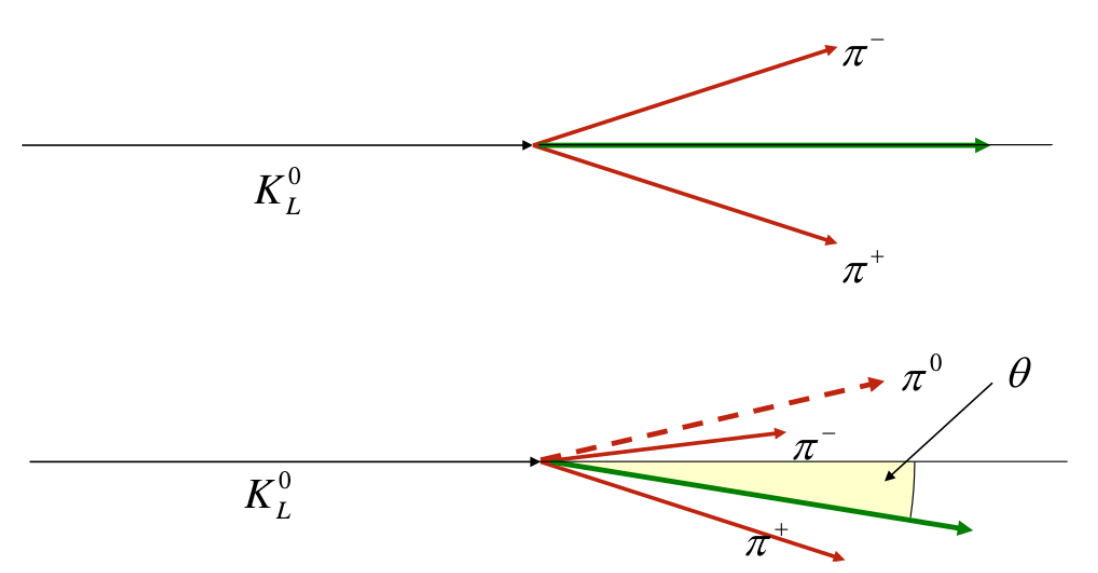
\includegraphics[height=6.0cm]{ressources/kaon.png}
  \caption{Messprinzip zur Unterscheidung von $2\pi$ und $3\pi$ Zerfällen \cite{kaon}.}
  \label{fig:kaon}
\end{figure}

Nachdem andere Effekte als Ursache ausgeschlossen werden konnten, bestätigte das Experiment 1964, dass es Zerfälle von $K_2^0$ Teilchen in $2\pi$ gibt.
Die vom Experiment beobachteten Teilchen entsprechen somit den Linearkombinationen
\begin{align*}
	\ket{K_\text{S}} &= \frac{1}{\sqrt{1+|\epsilon|^2}} \left( \ket{K_1} - \epsilon \ket{K_2} \right) \rightarrow \num{2} \pi  \\
	\ket{K_\text{L}} &= \frac{1}{\sqrt{1+|\epsilon|^2}} \left( \ket{K_2} + \epsilon \ket{K_1} \right) \rightarrow \num{3} \pi 
\end{align*}
wobei die Zerfälle für $\epsilon \neq 0$ CP-verletzend sind.
Der Parameter $\epsilon$ entspricht somit der CP-Verletzung in der Mischung.

%https://de.wikipedia.org/wiki/Kaon#Entdeckung

\subsection{CP-Verletzung in der Mischung und direkte CP-Verletzung}

Um die zeitliche Entwicklung des Kaonsystems zu beschreiben wird die Schrödingergleichung für $\ket{K^0(t)}$ und $\ket{\overline{K}^0(t)}$ aufgestellt und gelöst.
Hierbei führen Box-Diagramme höherer Ordnung zu Nebendiagonalelementen im Hamiltonian.
Durch das Diagonalisieren des Hamilotnian erhält man die bekannten Zustände $\ket{K_\text{S}}$ und $\ket{K_\text{L}}$.

Die CP-Verletzung in der Mischung tritt nun auf, wenn sich die Übergangswahrscheinlichkeiten von $K^0$ und $\overline{K}^0$ unterscheiden, d.h. 
\begin{align*}
	P\left( K^0 \rightarrow \overline{K}^0 \right) \neq P\left( \overline{K}^0 \rightarrow K^0 \right)
\end{align*}
erfüllt ist.

Zusätzlich kann auch eine direkte CP-Verletzung beobachtet werden, wenn 
\begin{align*}
	P\left( A \rightarrow B \right) \neq P\left( \overline{A} \rightarrow \overline{B} \right)
\end{align*}
für Kaonen erfüllt ist.
Während der Parameter für die CP-Verletzung in der Mischung $\epsilon$ heißt, existiert auch der Parameter $\epsilon^{\prime}$ welcher die direkte CP-Verletzung beschreibt.
In guter Näherung können diese Parameter über die Amplitudenverhältnisse von $K_\text{L}$- und $K_\text{S}$-Zerfällen in geladene bzw. ungeladene Pionen beschrieben werden.

Erste Messungen zur Suche nach direkter CP-Verletzung, welche deutlich seltener als indirekte CP-Verletzung in der Mischung zu messen ist, fanden 1988 am Experiment Na31 am CERN sowie N731 am Fermilab statt.
Aufgrund von fehlender Präzision lieferten diese Experiente noch keine signifikanten Ergebnisse.
Eine finale Bestätigung von direkter CP-Verletzung lieferte erst das Experiment Na48 am CERN.
Dieses Experiment konnte eine simultane Messung von $K_\text{L}$ und $K_\text{S}$ Zerfällen durchführen, insbesondere durch die Nutzung von Driftkammern sowie Kalorimetern zum Nachweis der Photonen im Zerfall neutraler Pionen.

\subsection{Ausblick}

Bis heute existieren Fragen im Bereich der CP-Verletzung.
Einerseits kann neben dem Kaon-System auch der B-Sektor und D-Sektor untersucht werden.
Andererseits ist eine CP-Verletzung innerhalb der starken Wechselwirkung in der Theorie erlaubt, konnte bisher jedoch noch nicht nachgewiesen werden.
Eine mögliche Lösung dieses sogenannten starken CP-Problems schlägt eine neue Symmetrie vor, aus der durch Symmetriebrechung das sogenannte Axion entsteht.
Dieses Teilchen, welches trotz intensiver Suchen noch nicht beobachtet wurde, wäre zusätzlich ein Kandidat für dunkle Materie.
